\section{Liang-Barsky裁剪算法}

\subsection{直线方程}

接下来首先写出直线的参数方程.。首先假定线段的起点$P_1$和终点$P_2$有如下坐标:

\begin{equation}
\begin{cases}
P_1 & (x_1, y_1) \\
P_2 & (x_2, y_2)
\end{cases}
\end{equation}

那么有直线的参数方程:

\begin{equation}
\begin{cases}
x = x_1+t(x_2-x_1) \\
y = y_1+t(y_2-y_1) 
\end{cases}
\end{equation}

其中$t$是参数。为了使方程归一化,将起始点与终点对应坐标相减作为斜率使用,这样,所有在线段上的点都满足:$0 \leq t \leq 1$。

\subsection{坐标系和裁剪要求}

为了使用Liang-Barsky裁剪,我们首先建立如下坐标系和裁剪要求:

\begin{figure}[H]
\centering
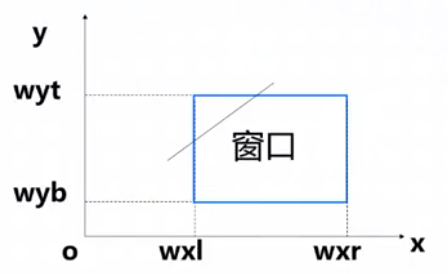
\includegraphics[width=0.8\textwidth,keepaspectratio]{imgs/lb-clip-co.png}
\end{figure}
 
其中$Y_{top}$为裁剪顶端,$Y_{bottom}$为裁剪底端,$X_{left}$为裁剪左侧,$X_{right}$为裁剪右侧。

那么一个位于窗口内的点,应满足如下不等式:

\begin{equation}
\begin{cases}
X_{left} \leq x \leq X_{right} \\
Y_{bottom} \leq y \leq Y_{top}
\end{cases}
\end{equation}

将直线的参数方程带入后有:

\begin{equation}
\begin{cases}
X_{left} \leq x_1+t(x_2-x_1) \leq X_{right} \\
Y_{bottom} \leq y_1+t(y_2-y_1) \leq Y_{top}
\end{cases}
\end{equation}

将连续不等式拆分成为单个不等式并移项后得:

\begin{equation}
\begin{cases}
t(x_1-x_2 ) & \leq x_1-X_{left} \\
t(x_2-x_1 ) & \leq X_{right}-x_1 \\
t(y_1-y_2 ) & \leq y_1-Y_{bottom} \\
t(y_2-y_1 ) & \leq Y_{top}-y_1
\end{cases}
\end{equation}

从上至下分别代表了左边界,右边界,下边界,上边界的约束。

\subsection{变量代换}

注意到以上不等式具有高度相似性,因此不妨做如下变量替换:

\begin{equation}
\begin{cases}
P_{left} & = x_1-x_2 \\
P_{right} & = x_2-x_1 \\
P_{bottom} & = y_1-y_2 \\
P_{top} & = y_2-y_1
\end{cases}
\qquad
\begin{cases}
Q_{left} & = x_1-X_{left} \\
Q_{right} & = X_{right}-x_1 \\
Q_{bottom} & = y_1-Y_{bottom} \\
Q_{top} & = Y_{top}-y_1
\end{cases}
\end{equation}

对于以上变换,我们将左侧统称为$P_{edge}$,右侧统称为$Q_{edge}$,其中$edge=left,right,bottom,top$。则上述不等式简化为:

\begin{equation}
t \cdot P_{edge} \leq Q_{edge}
\end{equation}

当不等号取等于时,求解出的t带入直线方程即可得到对应边的交点(包括延长线部分的交点)。我们将每个方程解出的对应的$t$值统称为$t_{edge}$。

\subsection{交点分组}

\begin{figure}[H]
\centering
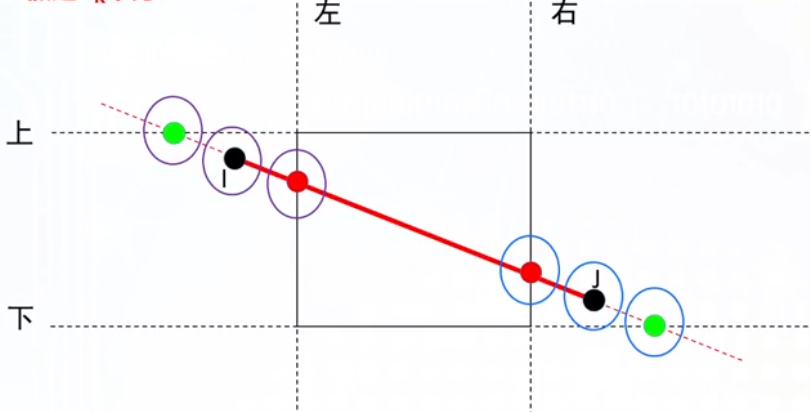
\includegraphics[width=0.8\textwidth,keepaspectratio]{imgs/lb-clip-intersection.png}
\end{figure}
 
首先假定$P_{edge} \neq 0$,即直线不与任何一条边平行(平行情况之后考虑)。那么Liang-Barsky裁剪要求我们将6个点(线段起点终点+4个交点)分成两组,一组表示进入窗口,另一组表示离开窗口。

Liang-Barsky裁剪指出,进入窗口组中的点,总是线段起点和满足$P_{edge}<0$的不等式所计算出的交点。而离开窗口组中的点,总是线段终点和满足$P_{edge}>0$的不等式所计算出的交点。由于$P_{edge}$表达式的对称性,$P_{edge}$中总是有2个正值,2个负值,因而它总是可以均分到两个组中,即每组三个点。

对于交点,我们可以根据不等式计算出其对应的$t_{edge}$。对于线段起点终点,其$t$值总为0和1。则在进入窗口组中,裁剪算法要求取$t$的最大值来计算交点。在离开窗口组中,裁剪算法要求取t的最小值来计算交点,即两者皆往线段中部收缩取值。总结如下:

\begin{equation}
\begin{cases}
t_{start} = \max ⁡(0,t_{edge},t_{edge}) & t_{edge}<0 \\
t_{end} = \min ⁡(1,t_{edge},t_{edge}) & t_{edge}>0
\end{cases}
\end{equation}

\subsection{额外约束}

当我们求解出$t_{start}$和$t_{end}$后,算法并没有结束。算法要求我们还需要保证如下不等式成立:

\begin{equation}
t_{start} \leq t_{end}
\end{equation}

如果不满足此不等式,则整条线段应当被舍弃。显而易见,我们获取到的裁剪后的线段的起点不应当越过线段的终点,因为我们定义的线段的参数方程中t时单调的,线段是有向的。而不满足此不等式的反例如下图所示:

\begin{figure}[H]
\centering
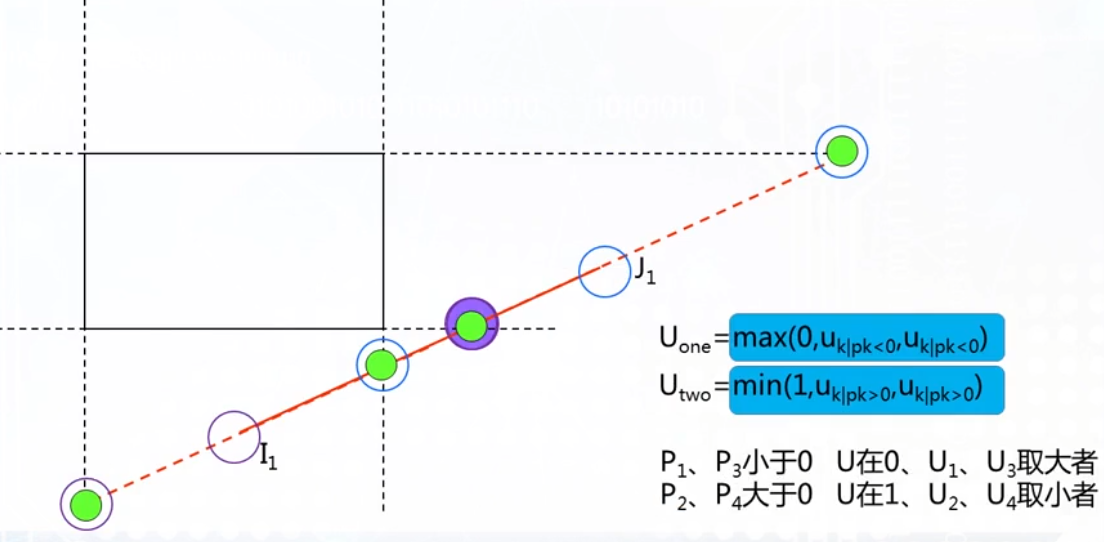
\includegraphics[width=0.8\textwidth,keepaspectratio]{imgs/lb-clip-invalid.png}
\end{figure}

即整条线段位于窗口之外,因此直接舍弃整条线段。

确认这一不等式成立后,对应$t$值就可以带入直线参数方程中,并计算出裁剪后的线段的起点和终点。

\subsection{特殊情况}

在前文中,我们假定$P_{edge} \neq 0$,即直线不与任何一条边平行。当部分$P_{edge}=0$时(不可能全部等于0,因为线段只能平行于一组边界),即线段与一组边界平行时,如下图所示。其中左图表示与左右边界平行,其$P_{left}=0,P_{right}=0$。右图表示与上下边界平行,其$P_{top}=0,P_{bottom}=0$。

\begin{figure}[H]
\centering
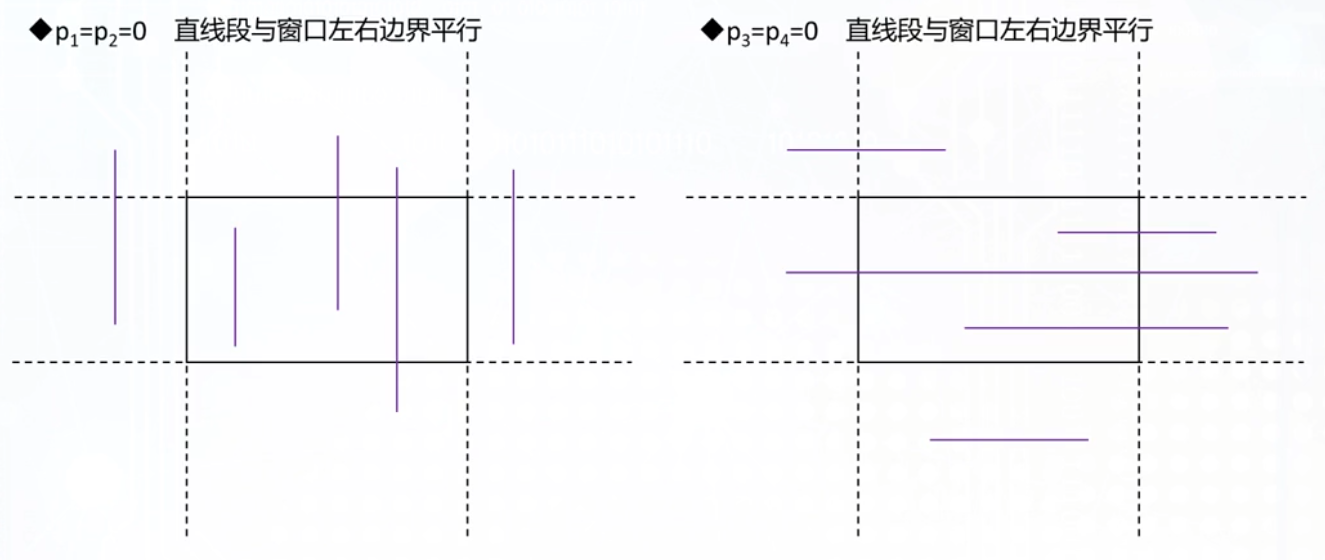
\includegraphics[width=0.8\textwidth,keepaspectratio]{imgs/lb-clip-special.png}
\end{figure}

显而易见,当线段与某一组边界平行时,这组平行的边界没有交点或有无数个交点,不能参与计算和使用,需要舍弃。
因此,Liang-Barsky裁剪要求,当$P_{edge}=0$时,对应不等式不参与解算,其不等式对应的交点不归入任何组中,也就是其对应的$t_{edge}$不参与最大值最小值计算(虽然是那么说,但是这个对应的$t_{edge}$实际上是解不出来的,因此当$P_{edge}=0$发现时就应当停止运算)。



